\subsection{Geometric element object -- ELE-GEO}
\label{sec:ele_geo}

As described in section \ref{sec:ovl}, the first step of finite
element analysis is the domain discretization. As a result we
obtain element meshes. Hereafter, we refer to a mesh element as
the geometric element object \texttt{ELE-GEO}. The intrinsic
properties of a geometric element object are: nodes, edges, faces, volume and neighbors (Fig. \ref{fig:elem}). Neighbor relationships connect
geometric element objects within a mesh and, therefore, represent
topological properties.

\begin{figure}[H]
\centering
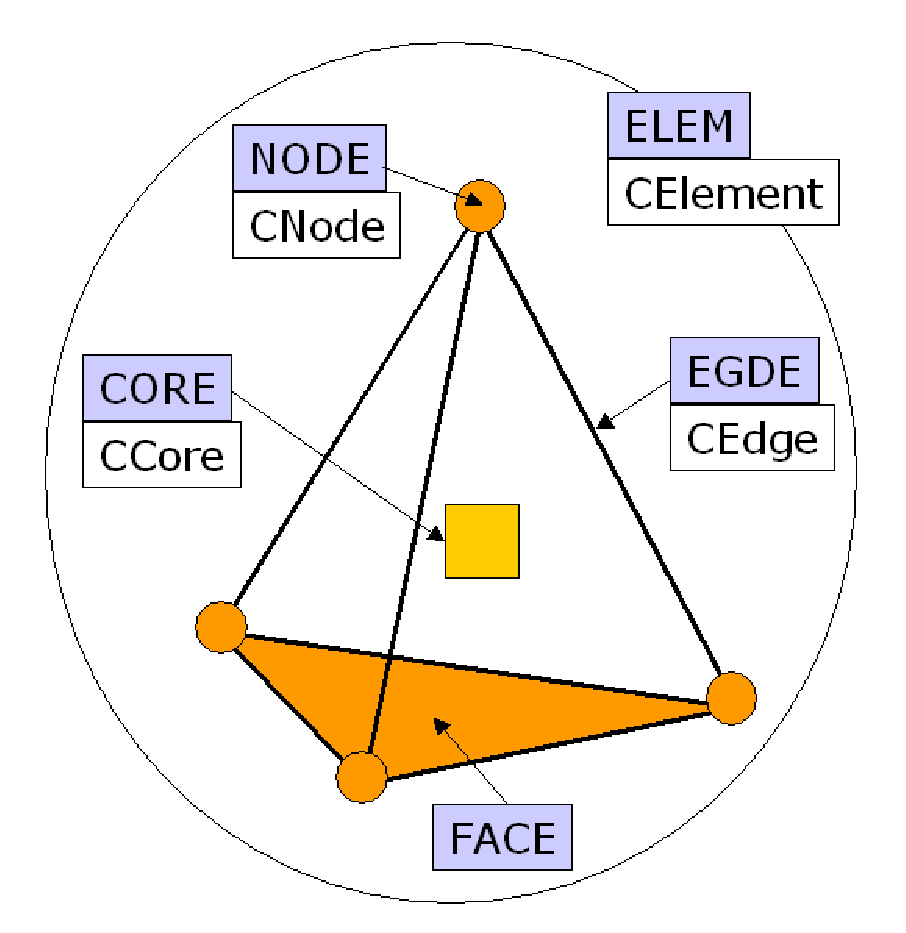
\includegraphics[scale=0.4]{figures/elem.eps}
\caption{Mesh element}
\label{fig:elem}
\end{figure}

%\begin{figure}[H]
%\centering
%\includegraphics[scale=0.7]{figure/gelement}
%\caption{Geometric element properties}
%\label{fig:gele}
%\end{figure}

We design the following element property classes to encapsulate
all geometric and topological element information.

\begin{itemize}
  \item \texttt{CCore} for \texttt{CORE} object,
  \item \texttt{CNode} for \texttt{NODE} object,
  \item \texttt{CEdge} for \texttt{EDGE} object,
  \item \texttt{CElem} for \texttt{ELEM} object.
\end{itemize}

Faces and neighbors belong to \texttt{ELEM} object. Indeed, edges
could be also assigned to the \texttt{ELEM} object. However, we
consider an edge as an individual entity for two reasons. First,
some numerical methods, such as mixed finite elements, require edges
as a basic geometric property as nodes for the Galerkin FEM. Second,
edges are frequently used as basic properties \rev{in automatic
generation}. As \texttt{NODE}, \texttt{EDGE} and \texttt{ELEM}
objects share common data and methods, we abstract these into the
\texttt{CCore} class as a base class.

\begin{figure}[H]
\centering
\shadowbox{
\begin{minipage}{0.9\textwidth}
{
\ttfamily \raggedright \small
\texttt{class\ CCore\\
\{\\
\ \ \ \textbf{protected}: // Properties\\
\ \ \ \ \ \ \textbf{long}\ index; // global element index\\
\ \ \ \ \ \ \textbf{char}\ position; // position indicator\\
%\ \ \ \ \ \ \textsl{//\ Status\ in\ usage}\\
\ \ \ \ \ \ \textbf{bool}\ status; //\ status\ in\ usage \\
%\ \ \ \ \ \ \textsl{//\ High\ order}\\
\ \ \ \ \ \ \textbf{int}\ order; // order of interpolation\\
\ \ \ \textbf{public}: // Methods\\
\ \ \ \ \ \ \textsl{//\ Set\ members}\\
\ \ \ \ \ \ \textbf{void}\ SetIndex(\textbf{const}\ \textbf{long}\ index)\ \{index\ =\ index;\}\\
\ \ \ \ \ \ \textbf{void}\ SetPosition(\textbf{const}\ \textbf{char}\ BC\underline\ type)\ \{boundary\ =\ BC\underline\ type;\}\\
\ \ \ \ \ \ \textbf{void}\ SetStatus(\textbf{const}\ \textbf{bool}\ status)\ \{status\ =\ status;\}\\
\ \ \ \ \ \ \textbf{void}\ SetOrder(\textbf{const}\ \textbf{int}\ order)\ \{order\ =\ order;\}\\
\ \ \ \ \ \ \textsl{//\ Get\ members}\\
\ \ \ \ \ \ \textbf{long}\ GetIndex()\ \textbf{const}\ \{\textbf{return}\ index;\}\ \\
\ \ \ \ \ \ \textbf{char}\ GetPosition()\ \textbf{const}\ \{\textbf{return}\ position;\}\ \\
\ \ \ \ \ \ \textbf{bool}\ GetStatus()\ \textbf{const}\ \{\textbf{return}\ status;\}\\
\ \ \ \ \ \ \textbf{int}\  GetOrder()\ \textbf{const}\ \{\textbf{return}\ order;\}\\
\ \ \ \ \ \ \textsl{//\ Construction}\\
\ \ \ \ \ \ CCore(\textbf{const}\ \textbf{int}\ id); // constructor\\
\ \ \ \ \ \ \textbf{virtual}\ \ \textasciitilde CCore(); // destructor\\
\ \ \ \ \ \ \textsl{//\ Operators}\\
\ \ \ \ \ \ \textbf{virtual}\ \textbf{void}\ \textbf{operator}\ =\ (\textbf{const}\ CCore\ \&\ g)\ \{\}\\
\ \ \ \ \ \ \textbf{virtual}\ \textbf{bool}\ \textbf{operator}\ ==\ (\textbf{const}\ CCore\ \&\ g)\ \{\textbf{return}\ \textbf{false};\}\\
\ \ \ \ \ \ \textsl{//\ Output}\\
\ \ \ \ \ \ \textbf{virtual}\ \textbf{void}\ output(ostream\&\ os=cout)\ \textbf{const}\ \{\};\\
\};\\
}
}
\normalfont\normalsize

\end{minipage}
}
\caption{\texttt{CCore} implementation for basic geometric element properties and methods}
\label{fig:core}
\end{figure}

\vfill

\newpage
%----------------------------------------------------------------------
\subsubsection{Core object - \texttt{CORE} - geometric element base class}
\label{sec:core}

Common data of a geometric element are: global element index;
position indicator within the whole domain, which indicates whether
the geometric element is inside the domain or on the domain surface;
%with specific boundary condition type;
status flag, which indicates whether this element is marked for
some usage. Assign $=$ as well as identity operators $==$ are
virtually defined. The C++ implementation of the \texttt{CCore} base
class is given in Fig. \ref{fig:coree}.

\begin{figure}[H]
\centering
\includegraphics[scale=0.4]{figures/core.eps}
\caption{Core of mesh element} \label{fig:coree}
\end{figure}

\rev{Member \mbox{\texttt{char position}} is used to determine the
location of the geometrical entity within a domain, e.g. it is
inside the domain or on the boundary of the domain.}
%%\input{code/core}

Classes \texttt{CNode}, \texttt{CEdge} and \texttt{CElem} are
directly derived from the base class \texttt{CCore}. Assign $=$ as
well as the identity operator $==$ are overloaded in these
objects. With such overloading operators, passing data of an class
instance, \texttt{A}, to another class instance, \texttt{B}, can
be simply realized with the instruction
\mbox{\texttt{A}=\texttt{B}}. Whether two instances are identical
can be checked by the instruction
\mbox{\texttt{if}(\texttt{A}==\texttt{B})}.

\begin{figure}[H]
\centering
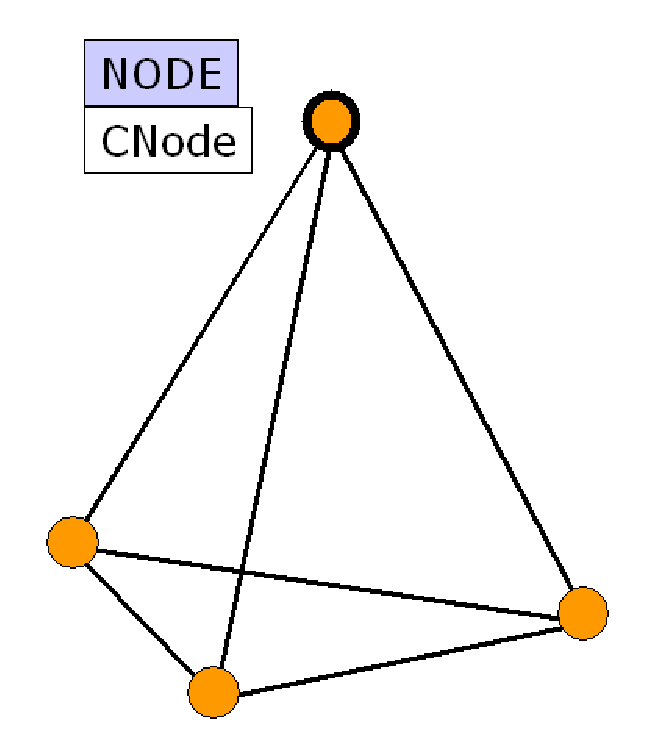
\includegraphics[scale=0.4]{figures/node.eps}
\caption{Node of element object} \label{fig:node1}
\end{figure}

%----------------------------------------------------------------------
\subsubsection{Node object - \texttt{NODE}}
\label{sec:node}

The node object (\texttt{NODE}) is derived from the \texttt{CCore}
class. In addition, the \texttt{CNode} class provides the
geometrical position of an element in real space, i.e. the coordinates
of element nodes (Fig. \ref{fig:node1}).

\begin{figure}[H]
\centering
\shadowbox{
\begin{minipage}{0.95\textwidth}
{\sffamily \raggedright
\footnotesize \texttt{class\ CNode:\textbf{public}\ CCore\\
\{\\
\ \ \ \textbf{private}: // Members\\
\ \ \ \ \ \ \textbf{double}\ coordinate[3];\\
\ \ \ \ \ \ Vector$<${}\textbf{long}$>${} ConnectedElements;\ \ \ \\
\ \ \ \ \ \ \rev{Vector$<${}\textbf{long}$>${} ConnectedNodes;}\ \ \ \\
\ \ \ \textbf{public}:\\
\ \ \ \ \ \ \textsl{//\ Construction}\\
\ \ \ \ \ \ Node(\textbf{const}\ \textbf{int}\ Index,\ \textbf{const}\ \textbf{double}\ x,\ \\
\ \ \ \ \ \ \ \ \ \ \ \textbf{const}\ \textbf{double}\ y,\ \textbf{const}\ \textbf{double}\ z=0.0);\\
\ \ \ \ \ \ Node()\ \{\}\\
\ \ \ \ \ \ \textasciitilde Node()\ \{ConnectedElements.resize(0); ConnectedNodes.resize(0);\}\\
\ \ \ \ \ \ \textsl{//\ Operators}\\
\ \ \ \ \ \ \textbf{void}\ \textbf{operator}\ =\ (\textbf{const}\ Node\&\ n);\\
\ \ \ \ \ \ \textbf{bool}\ \textbf{operator}\ ==\ (\textbf{const}\ Node\ \&\ n);\\
\ \ \ \ \ \ \textsl{//\ Set members}\\
\ \ \ \ \ \ \textbf{void}\ SetX(\textbf{const}\ \textbf{double}\ argX)\ \{\ coordinate[0]\ =\ argX;\}\\
\ \ \ \ \ \ \textbf{void}\ SetY(\textbf{const}\ \textbf{double}\ argY)\ \{\ coordinate[1]\ =\ argY;\}\\
\ \ \ \ \ \ \textbf{void}\ SetZ(\textbf{const}\ \textbf{double}\ argZ)\ \{\ coordinate[2]\ =\ argZ;\}\\
\ \ \ \ \ \ \textbf{void}\ SetCoordinates(\textbf{const}\ \textbf{double}$\ast$\ argCoord);\ \\
\ \ \ \ \ \ \textsl{//\ Get members}\\
\ \ \ \ \ \ \textbf{double}\ GetX()\ \textbf{const}\ \{\textbf{return}\ coordinate[0];\}\\
\ \ \ \ \ \ \textbf{double}\ GetY()\ \textbf{const}\ \{\textbf{return}\ coordinate[1];\}\\
\ \ \ \ \ \ \textbf{double}\ GetZ()\ \textbf{const}\ \{\textbf{return}\ coordinate[2];\}\\
%\ \ \ \ \ \ \textbf{void}\ Coordinates(\textbf{double}\ $\ast$xyz)\ \textbf{const}\\
%\ \ \ \ \ \ \{\ \ \textbf{for}(\textbf{int}\ i=0;\ i$<${}3;\ i++)\ \ xyz[i]\ =\ Coordinate[i];\}\ \\
\ \ \ \ \ \ \textbf{int}\ GetNumberOfConnectedElements()\ \textbf{const}\ \{\textbf{return}\ ConnectedElements.size();\ \}\ \ \ \ \ \\
\ \ \ \ \ \ \rev{\textbf{int}\ GetNumberOfConnectedNodes()\ \textbf{const}\ \{\textbf{return}\ ConnectedNodes.size();}\ \}\ \ \ \ \ \\
\ \ \ \ \ \ \textsl{//\ Output}\\
\ \ \ \ \ \ \textbf{void}\ Write(ostream\&\ os=cout)\ \textbf{const};\\
\ \ \ \textbf{private}: // Class relations\\
\ \ \ \ \ \ \textbf{friend}\ \textbf{class}\ CEdge;\\
\ \ \ \ \ \ \textbf{friend}\ \textbf{class}\ CElem;\\
\};\\
}
 }
\normalfont\normalsize

\end{minipage}
}
\caption{\texttt{CNode} implementation}
\label{fig:node}
\end{figure}

Mesh elements having this node in common are determined immediately
after mesh data is generated. Elements sharing this node are stored
in vector \texttt{ConnectedElements}. This node-element relationship
is very important information of the mesh topology. It is required
e.g. for extrapolation of Gauss point values to node values or for
projecting element properties to nodes. Using the
\texttt{ConnectedElements} vector, the calculation of mesh topology
can be enormously accelerated. \rev{For extrapolation of gauss point
values to nodes, we only need to know the size of the vector, i.e.
how many element connected to the nodes. Since extrapolation takes
place in element-wise, node values are accumulated from the
contribution of its connected elements, we have to average the
accumulated node value by dividing it with the number of connected
elements after extrapolation is finished. Member vector
\texttt{ConnectedNodes} stores indices of all nodes of connected
elements and it used together with the degree of freedom of the
preocess/problem to store indices of all nodes of connected elements
and it can be used together with the degree of freedom of the
preocess/problem to create the sparse matrix of the system
equations.to create the sparse matrix of the system equations. The
memory of \texttt{ConnectedNodes} is released as soon as the sparse
matrix is created.} Classes \texttt{CEdge} and \texttt{CElem} are
set as friend classes of \texttt{CNode} so that they can access to
\texttt{CNode} private members directly. The C++ implementation of
\texttt{class CNode} is given in Fig. \ref{fig:node}.

Instances of \texttt{NODE} object are stored in a global vector: \\
\texttt{vector<CNode*>node\_vector}.

%----------------------------------------------------------------------
\subsubsection{Edge object - \texttt{EDGE}}
\label{sec:edge}

The edge object (\texttt{EDGE}) is derived from the \texttt{CCore}
class. Edges are used to build up the frame of a geometric element
object (Fig. \ref{fig:gedge}). It is sufficient to use two nodes to
form a geometric edge. However, for higher order finite elements,
more points are required along an edge. Therefore, we use a vector
of \texttt{CNode} pointers as class member for edge nodes (see Fig.
\ref{fig:gedge}). In case of quadratic finite elements, the first
two nodes are element corner nodes and the last one is the middle
point of this edge.

\begin{figure}[H]
\centering
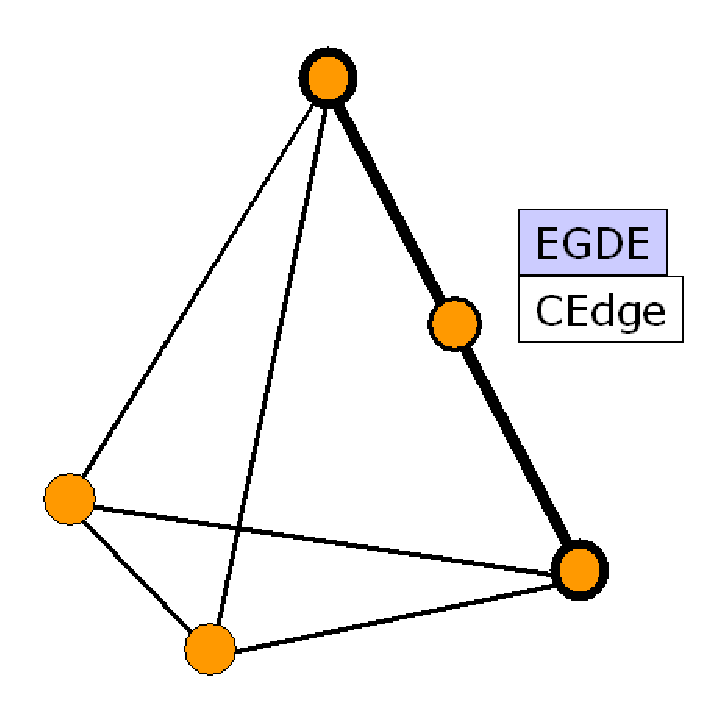
\includegraphics[scale=0.4]{figures/edge_new.eps}
\caption{Edge of mesh element} \label{fig:gedge}
\end{figure}

The C++ implementation of the \texttt{CEdge} class is given in
Fig. \ref{fig:edge}.

\texttt{Vector} is a "clone" of the standard C++ vector template,
as \texttt{template Vector\-<class V> class V} with less memory consuming but sufficient
and efficient functionality of vector algebraic calculation.

For node based finite elements (i.e. linear
interpolation), edges are only used to the compute topological mesh
structure \rev{and to process Dirichlet  boundary conditions and
source terms. For instance, if a Dirichlet  boundary condition of a
PDE is assigned by a polyline, edges of elements on the polyline
will be found and the Gauss integration will be performed on these
edges to produce node values of nodes of these edges}. They are not
needed to be stored for the later computations anymore. On the other
hand, mixed finite elements or higher order finite elements require
edges through all computations. In this case we save all edges of a
mesh in a standard C++ vector: \texttt{vector<CEdge*>egde\_vector}.

\begin{figure}[H]
\centering
\shadowbox{
\begin{minipage}{0.95\textwidth}
{
\sffamily \raggedright \scriptsize
\texttt{class\ CEdge:\textbf{public}\ CCore\\
\{\\
\ \ \ \textbf{private}: // Members\\
\ \ \ \ \ \ vec$<${}CNode$\ast>${}\ nodes\underline\ of\underline\ edges;\\
\ \ \ \textbf{public}: // Member functions\\
\ \ \ \ \ \ \textsl{//\ Construction}\\
\ \ \ \ \ \ Edge(\textbf{const}\ \textbf{int}\ Index,\ \textbf{bool}\ quadr=\textbf{false});\\
\ \ \ \ \ \ \textasciitilde Edge();\ \\
\ \ \ \ \ \ \textsl{//\ Operators}\\
\ \ \ \ \ \ \textbf{void}\ \textbf{operator}\ =\ (CEdge\&\ edg);\\
\ \ \ \ \ \ \textbf{bool}\ \textbf{operator}\ ==\ (CEdge\&\ edg);\\
\ \ \ \ \ \ \textsl{//\ Member access}\\
\ \ \ \ \ \ \textbf{void}\ SetNodes(\ vec$<${}CNode$\ast>${}\&\ Nodes)\\
\ \ \ \ \ \ \{\ \textbf{for}(\textbf{int}\ i=0;\ i$<${}(\textbf{int})Nodes.Size();\ i++)\ \ Nodes[i]\ =\ nodes\underline\ of\underline\ edges[i];\ \}\\
\ \ \ \ \ \ \textbf{void}\ SetNodes(\ vec$<${}CNode$\ast>${}\&\ Nodes)\ \textbf{const}\ \{\ Nodes\ =\ nodes\underline\ of\underline\ edges;\}\\
\ \ \ \ \ \ \textsl{//\ Output}\\
\ \ \ \ \ \ \textbf{void}\ Write(ostream\&\ osm=cout)\ \textbf{const};\\
\ \ \ \textbf{private}: // Class relations\\
\ \ \ \ \ \ Vector$<${}CNode$\ast>${}\ \ nodes\underline\ of\underline\ edges;\\
\ \ \ \ \ \ \textbf{friend}\ \textbf{class}\ CElem;\\
\};\\
}
 }
\normalfont\normalsize

\end{minipage}
}
\caption{\texttt{CEdge} implementation}
\label{fig:edge}
\end{figure}

%
\begin{figure}[H]
\centering
\shadowbox{
\begin{minipage}{0.9\textwidth}
{
\sffamily \raggedright \scriptsize
\texttt{class\ CElement:\textbf{public}\ CCore\\
\{\\
\ \ \ \textbf{private}:\ \textsl{//\ Members}\\
\ \ \ \ \ \ \textsl{//\ ID}\\
\ \ \ \ \ \ CElem$\ast$\ owner;\\
\ \ \ \ \ \ \textbf{int}\ ele\underline\ type;\ \ \textsl{//\ Element\ type}\\
\ \ \ \ \ \ \textsl{//\ Geometrical properties}\\
\ \ \ \ \ \ \textbf{int}\ dim;\ \ \ \ \ \ \ \textsl{//\ dimension\ of\ element}\\
\ \ \ \ \ \ \textbf{double}\ volume;\ \textsl{// element volume}\\
\ \ \ \ \ \ \textsl{//\ Topological properties}\\
\ \ \ \ \ \ \textbf{int}\ nnodes;\ \ \ \ \textsl{//\ number\ of element corner nodes}\\
\ \ \ \ \ \ \textbf{int}\ nnodesHQ;\ \ \textsl{//\ number of element nodes for quadratic interpolation}\\
\ \ \ \ \ \ Vector$<${}CNode$\ast>${}\ \ nodes;\\
\ \ \ \ \ \ \textbf{int}\ nedges;\ \ \ \ \textsl{//\ number\ of\ edges}\\
\ \ \ \ \ \ Vector$<${}CEdge$\ast>${}\ \ edges;\\
\ \ \ \ \ \ \textbf{int}\ nfaces;\ \ \ \ \textsl{//\ number\ of\ faces}\\
\ \ \ \ \ \ \textsl{//\ Mesh topology}\\
\ \ \ \ \ \ \textbf{int}\ sub\_domain;\\
\ \ \ \ \ \ Vector$<${}CElem$\ast>${}\ \ neighbors;\\
\ \ \ \ \ \ Vector$<${}CElem$\ast>${}\ \ sons;\\
%%\ \ \ \ \ \ \textsl{//\ ???}\\%%
\ \ \ \ \ \ Vector$<${}\textbf{long}$>${}\ \ \ nodes\underline\ index;\\
\}\\
}
 }
\normalfont\normalsize

\end{minipage}
}
\caption{\texttt{CElem} implementation}
\label{fig:gelee}
\end{figure}
%

%----------------------------------------------------------------------
\subsubsection{Element object - \texttt{ELEM}}
\label{sec:elem}

The element object (\texttt{ELEM}) is also derived from the
\texttt{CCore} class. \texttt{ELEM} represents an individual
element of a mesh. Node and edge objects are employed to construct
the element object. An abstract mesh element object is designed
for different geometric element types, i.e. lines, triangles,
quadrilaterals, tetrahedra, triangle based prisms, hexahedra
(Table \ref{tab:elem}, Fig. \ref{fig:ele_types}). These geometric
element types are defined by an ID, i.e, integer number represent
element type.
The C++ implementation of \texttt{class CElem} is given in Fig.
\ref{fig:gelee}.

Basic members of the element object are identification,
geometrical as well as topological properties and mesh
relationships.
%
Element ID (index) is inherited from the \texttt{CORE} object.
Dimension and volume are basic geometric members. Depending on the
geometric type of an element (\texttt{ele\_type}), the following
 geomatrical and topological properties are specified:

\begin{table}[H]
\caption{Basic topology information of an geometrical element}
\begin{center}
% use packages: array
\begin{tabular}{lccccc}
\hline
Geometric type  & \texttt{ele\_type}&\texttt{nnodes}& \texttt{nnodesHQ}& \texttt{nfaces} & \texttt{nedges}\\
\hline
Line &1& 2&3& &\\
Quadrilateral&2&4&9& 4&4\\
Hexehedron&3& 8&20& 6&12\\
Triangle&4&  3&6& 3&3\\
Tetrahedron & 5& 4&10& 4&6\\
Prism &6  & 6&15& 5&9\\
\hline
\label{tab:elem}
\end{tabular}
\end{center}
\end{table}


Element nodes and edges are kept in the following two member vectors

\texttt{$\quad$Vector$<${}CNode$\ast>${}\ nodes;} 

and

\texttt{$\quad$Vector$<${}CEdge$\ast>${}\ edges;}

%The element configuration is conducted based on the geometric
%element type with member function {\texttt{CElem::Config(long
%element\_index}}. By this the corresponding \texttt{ELEM} members
%are created and initialized (Table \ref{tab:elem}).

\begin{figure}[htb!]
\centering
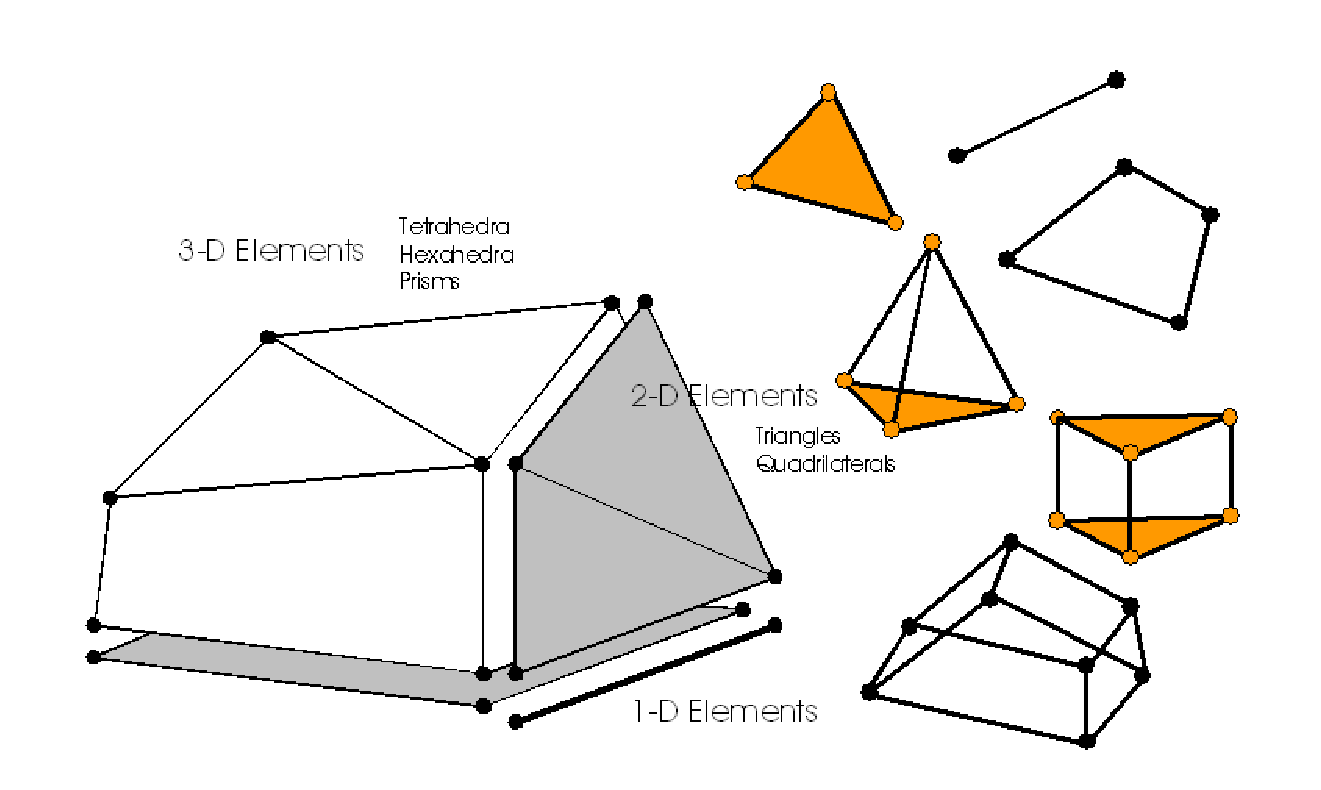
\includegraphics[scale=0.55]{figures/elements.eps}
\caption{Geometric elements types} \label{fig:ele_types}
\end{figure}
